\documentclass[11pt]{article}
\usepackage{amsmath,amssymb,graphicx,xcolor,tikz}
\usetikzlibrary{arrows.meta,calc,positioning}
\newcommand{\M}{\mathcal M}
\newcommand{\R}{\mathbb R}
\newcommand{\T}{\mathsf T}
\newcommand{\Wwin}{\mathcal W}
\newcommand{\Hscore}{\mathcal H}
\DeclareMathOperator{\reach}{reach}
% Numbering in the submitted manuscript.
\makeatletter
\newlabel{prop:pilot}{{3.1}{}}
\newlabel{prop:step}{{3.2}{}}
\newlabel{prop:finite}{{3.3}{}}
\newlabel{prop:readout}{{3.4}{}}
\newlabel{thm:isolated-rank}{{3.5}{}}
\makeatother
\pagestyle{empty}
\begin{document}
\setbox0=\hbox\bgroup
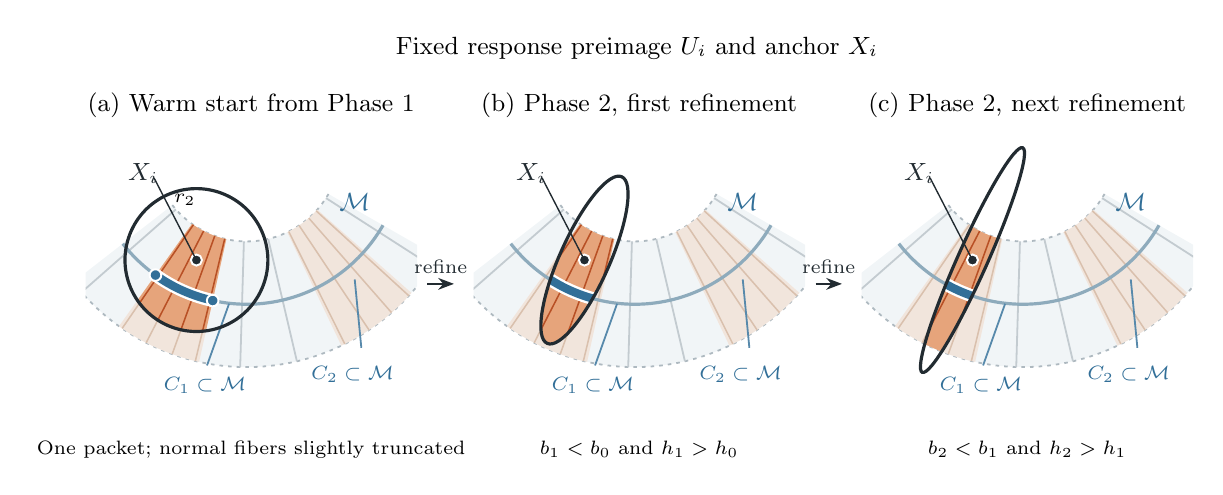
\begin{tikzpicture}[x=.028cm,y=.028cm,>=Stealth]
% Match the palette and geometry of MFM_m2_response_preimage.pdf exactly.
% Coordinates are centered at the common center of the three circular arcs
% in that figure's middle panel; one coordinate unit is one PDF point.
\definecolor{phaseblue}{RGB}{50,111,152}
\definecolor{phasethinblue}{RGB}{142,171,188}
\definecolor{phaselightblue}{RGB}{241,245,247}
\definecolor{phaseblueedge}{RGB}{174,185,192}
\definecolor{phasefiber}{RGB}{195,203,208}
\definecolor{phaseorange}{RGB}{230,164,123}
\definecolor{phaseorangeedge}{RGB}{184,80,37}
\definecolor{phasetan}{RGB}{241,229,220}
\definecolor{phasetanedge}{RGB}{217,192,173}
\definecolor{phaseblack}{RGB}{34,43,49}

\newcommand{\phaseannulus}[3]{%
  \path[fill=#3,draw=none]
    ({99.75*cos(#1)},{99.75*sin(#1)})
    arc[start angle=#1,end angle=#2,radius=99.75]
    -- ({42.75*cos(#2)},{42.75*sin(#2)})
    arc[start angle=#2,end angle=#1,radius=42.75] -- cycle;
}

\newcommand{\phasepacketfibers}[2]{%
  \foreach \aa in {#1}
    \draw[#2,line width=.55pt]
      ({99.75*cos(\aa)},{99.75*sin(\aa)}) --
      ({42.75*cos(\aa)},{42.75*sin(\aa)});
}

\newcommand{\phasepackets}[2]{%
  \phaseannulus{-125.5}{-102.5}{#1}
  \phaseannulus{-64.5}{-41.5}{#1}
  \phasepacketfibers{-124.5,-117.2,-109.8,-103.5}{#2}
  \phasepacketfibers{-63.5,-56.2,-48.8,-42.5}{#2}
}

\newcommand{\phasesection}{%
  \begin{scope}
    \clip (-73.03,-107.23) rectangle (77.31,-12.47);
    \phaseannulus{-142.1}{-29.8}{phaselightblue}
    \draw[phaseblueedge,dash pattern=on 1.3pt off 1.82pt,line width=.65pt]
      ({99.75*cos(-142.1)},{99.75*sin(-142.1)})
      arc[start angle=-142.1,end angle=-29.8,radius=99.75];
    \draw[phaseblueedge,dash pattern=on 1.3pt off 1.82pt,line width=.65pt]
      ({42.75*cos(-142.1)},{42.75*sin(-142.1)})
      arc[start angle=-142.1,end angle=-29.8,radius=42.75];
    \foreach \aa in {-138.7,-91.7,-76.8,-32.7}
      \draw[phasefiber,line width=.65pt]
        ({99.75*cos(\aa)},{99.75*sin(\aa)}) --
        ({42.75*cos(\aa)},{42.75*sin(\aa)});
    \phasepackets{phasetan}{phasetanedge}
  \end{scope}
}

\newcommand{\phasemanifold}{%
  \draw[phasethinblue,line width=1.15pt]
    ({71.25*cos(-142.1)},{71.25*sin(-142.1)})
    arc[start angle=-142.1,end angle=-29.8,radius=71.25];
  \node[phaseblue,font=\small] at (49,-25) {$\mathcal M$};
  \draw[phaseblue!82,line width=.65pt] (-18,-99) -- (-8,-71);
  \node[phaseblue,font=\scriptsize] at (-19,-108) {$C_1\subset\mathcal M$};
  \draw[phaseblue!82,line width=.65pt] (52,-91) -- (49,-60);
  \node[phaseblue,font=\scriptsize] at (48,-103) {$C_2\subset\mathcal M$};
}

\newcommand{\phasepacketmanifold}{%
  % The heavy part is clipped below to the displayed neighborhood; the
  % remainder of the manifold therefore retains Figure 2's thin stroke.
  \foreach \lo/\hi in {-125.5/-102.5,-64.5/-41.5}{%
    \draw[white,line width=4.7pt]
      ({71.25*cos(\lo)},{71.25*sin(\lo)})
      arc[start angle=\lo,end angle=\hi,radius=71.25];
    \draw[phaseblue,line width=3pt]
      ({71.25*cos(\lo)},{71.25*sin(\lo)})
      arc[start angle=\lo,end angle=\hi,radius=71.25];
    \filldraw[fill=phaseblue,draw=white,line width=.7pt]
      ({71.25*cos(\lo)},{71.25*sin(\lo)}) circle[radius=2.1pt];
    \filldraw[fill=phaseblue,draw=white,line width=.7pt]
      ({71.25*cos(\hi)},{71.25*sin(\hi)}) circle[radius=2.1pt];
  }
}

\newcommand{\phaseneighborhood}[2]{%
  \begin{scope}
    \clip[rotate around={-24.1:(-22.80,-51.20)}]
      (-22.80,-51.20) ellipse[x radius=#1,y radius=#2];
    \begin{scope}
      \clip (-73.03,-107.23) rectangle (77.31,-12.47);
      \phasepackets{phaseorange}{phaseorangeedge}
    \end{scope}
  \end{scope}
  \phasemanifold
  \begin{scope}
    \clip[rotate around={-24.1:(-22.80,-51.20)}]
      (-22.80,-51.20) ellipse[x radius=#1,y radius=#2];
    \phasepacketmanifold
  \end{scope}
  \draw[phaseblack,line width=1.15pt,
        rotate around={-24.1:(-22.80,-51.20)}]
    (-22.80,-51.20) ellipse[x radius=#1,y radius=#2];
  \filldraw[fill=phaseblack,draw=white,line width=.7pt]
    (-22.80,-51.20) circle[radius=2pt];
  \draw[phaseblack,line width=.5pt] (-22.80,-51.20) -- (-42,-14);
  \node[phaseblack,font=\small] at (-47,-12) {$X_i$};
}

\newcommand{\phasepanel}[5]{%
  \begin{scope}[shift={(#1,0)}]
    \node[font=\small] at (2,19) {#2};
    \phasesection
    \phaseneighborhood{#3}{#4}
    \node[font=\scriptsize,align=center] at (2,-137) {#5};
  \end{scope}
}

  \node[font=\small] at (177,45)
    {Fixed response preimage $U_i$ and anchor $X_i$};%
  % The first panel uses the circular-arc geometry of Figure 2(b),
  % with an intermediate scan radius of 32.4.
  \phasepanel{0}{(a) Warm start from Phase~1}{32.4}{32.4}
    {One packet; normal fibers slightly truncated}
  \node[font=\scriptsize] at (-28,-24) {$r_2$};
  \phasepanel{176}{(b) Phase~2, first refinement}{11.25}{41.4}
    {$b_1<b_0$ and $h_1>h_0$}
  \phasepanel{352}{(c) Phase~2, next refinement}{6.75}{55.8}
    {$b_2<b_1$ and $h_2>h_1$}
  \draw[-{Stealth[length=2mm]},phaseblack,line width=.65pt]
    (82,-62) -- node[above,font=\scriptsize] {refine} (94,-62);
  \draw[-{Stealth[length=2mm]},phaseblack,line width=.65pt]
    (258,-62) -- node[above,font=\scriptsize] {refine} (270,-62);
\end{tikzpicture}
\egroup
\pdfpagewidth=\dimexpr\wd0+4pt\relax
\pdfpageheight=\dimexpr\ht0+\dp0+4pt\relax
\hoffset=-1in \voffset=-1in
\shipout\vbox{\kern2pt\hbox{\kern2pt\box0}}
\end{document}
